\chapter{Introduzione}
\section{Terminologia di base}
Per avere un'implementazione corretta e completa del software dobbiamo fare 
in modo che il software risolva un problema concreto del mondo reale. Dobbiamo quindi 
comprendere correttamente il mondo reale, ovvero come funziona, come dovrebbe 
funzionare, quali sono i vincoli che governano, capire il contesto in cui il
software deve operare. Questo è il compito dell'ingegneria dei requisiti.

\subsubsection{Esempio}
\begin{itemize}
        \item \textbf{Problema}: la gestione del freno a mano in un'automobile 
        moderna potrebbe essere automatizzato.
        \item \textbf{Contesto}: se l'automobile è in movimento, 
        se si sta frenando, se è intenzione del guidatore fermarsi,
        se il guidatore ha premuto il pedale del freno, \dots
\end{itemize}

Quando parliamo di \textbf{requisiti} dobbiamo inoltre definire il 
\textbf{mondo}. Quando definiamo il mondo, abbiamo a che fare con elementi molto 
complessi che contengono di fatto elementi umani (\textit{lo staff, 
l'utente, il cliente, \dots}), elementi fisici (\textit{dispositivi, 
software legacy, la natura, \dots}) e dovrà quindi adattarsi alla situazione 
esistente.

Dobbiamo definire anche il mondo delle \textbf{macchine}. Parliamo 
quindi di tutto ciò che dovrà essere implementato e/o acquistato, come ad esempio
\textit{database, server, client, \dots} e i componenti 
hardware e software che dovranno essere implementati.

L'ingegneria dei requisiti non si limita solamente al mondo delle 
macchine, ma tiene in considerazione anche gli effetti che il 
software ha sul mondo reale, che dovrà modellare. 

Il mondo e le macchine hanno i propri fenomeni, ma ne condividono 
anche alcuni. Ad esempio, il mondo ha il \textit{rilascio del freno a mano},
mentre le macchine hanno \texttt{errorCode = 013}. Nell'intersezione 
potremmo avere ad esempio \texttt{motor.Regime =`up`}.
\begin{figure}[H]
    \centering
    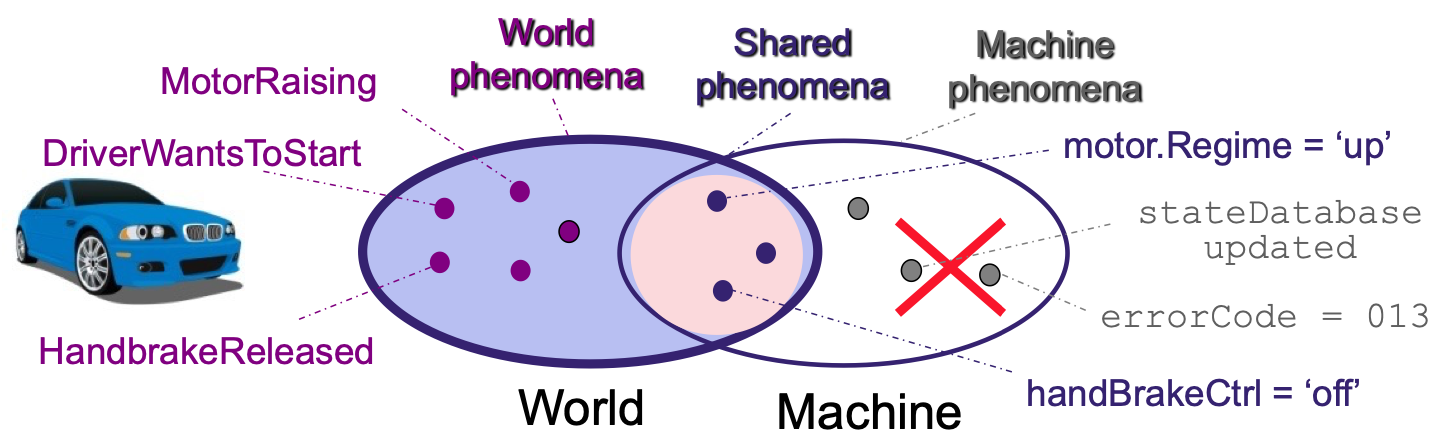
\includegraphics[scale=0.3]{img/worldmod.png}
    \caption{Il mondo e le macchine}
    \label{fig:req_eng}
\end{figure}
\begin{tcolorbox}[colback=green!5!white,colframe=green!75!black]
    Quando parliamo di requisiti, consideriamo solamente la parte 
    relativa al mondo, che comprende quindi anche l'intersezione.
    È importante comprendere che non descrivono \textbf{nulla}
    riguardo alle macchine.
\end{tcolorbox}
\subsection{Le due versioni del mondo}
Il sistema è l'insieme delle interazioni delle componenti che 
strutturano il mondo.
\begin{itemize}
    \item Il sistema \textbf{as-is}: si tratta del sistema prima che 
    il software venga implementato. Questo sistema è composto da
    solamente dal mondo.
    \item Il sistema \textbf{to-be}: si tratta del sistema come 
    dovrebbe essere quando il software opererà. Questo sistema
    è composto dall'unione del mondo e delle macchine.
\end{itemize}
\begin{tcolorbox}[title=Definizione preliminare dell'ingegneria dei requisiti,
colback=blue!5!white,colframe=blue!75!black]
    Consiste in una serie di attività collegate tra loro che ci permettono 
    di esplorare, valutare, documentare, consolidare, rivedere e adattare 
    quelli che sono gli obiettivi, le capacità, i vincoli e le assunzioni 
    in un sistema software. Basato sui problemi del sistema \textbf{as-is}
    e le opportunità date dalle nuove tecnologie.
\end{tcolorbox}

\subsection{I requisiti di sistema e i requisiti software}
Il sistema (\textit{unione del mondo reale e del sistema software}) sono 
i requisiti che fanno riferimento a tutto, si tratta degli statement che 
fanno parte del \textbf{system to-be}, mentre i requisiti software
sono un sottoinsieme dei requisiti di sistema, fanno quindi riferimento
solamente al \textbf{software to-be}, di fatto le funzionalità che il software 
che dovrà fornire per rispondere in maniera adeguata ai 
problemi del nostro utente.

\section{Scope dell'ingegneria dei requisiti}
\begin{figure}[H]
    \centering
    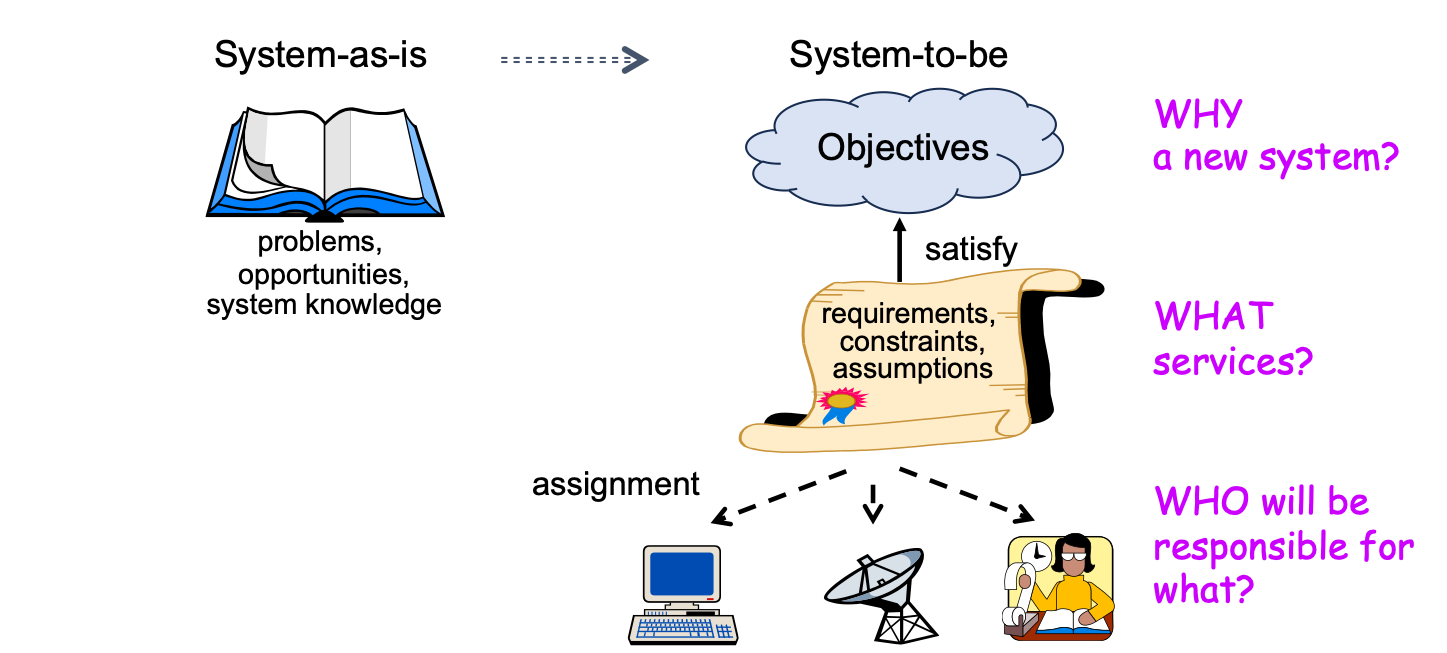
\includegraphics[scale=0.3]{img/scope.png}
    \caption{Scope dell'ingegneria dei requisiti}
    \label{fig:scope}
\end{figure}
Prima di iniziare a lavorare sui requisiti, abbiamo il nostro 
system as-is, che comprenderà i problemi, le opportunità e le 
conoscenze sul sistema. Da qui mapperemo il tutto nel 
system to-be. Per comprendere al meglio il system to-be,
dobbiamo ragionare in tre prospettive:
\begin{itemize}
    \item Perché: quali sono gli obiettivi dell'abbinamento 
    tra software e mondo reale. Quindi quali sono le necessità 
    che il software dovrà soddisfare.
    \item Cosa: quali sono le funzionalità che il software dovrà
    fornire per soddisfare i bisogni del cliente, quali saranno i 
    vincoli e le assunzioni che il software dovrà rispettare.
    \item Chi: chi sarà responsabile della fornitura 
    delle funzionalità.
\end{itemize}
Questa è la chiave di lettura quando ragioniamo in termini 
di software: dobbiamo capire quali sono le funzionalità esposte e come 
queste danno una risposta agli obiettivi che ci siamo posti e 
chi ha la responsabilità di implementare tali funzionalità, se una persona,
un componente interno al sistema, un componente esterno, \dots.
Ci saranno quindi delle viste diverse che ci permetteranno di ragionare 
in questo spazio tridimensionale.
\subsection{La dimensione del perché}
Si tratta dell'identificazione degli obiettivi di cui il 
sistema software dovrà dare risposta. Vanno identificati, perciò 
l'interazione con gli stakeholder è essenziale, ma vanno inoltre 
analizzati. Tali obiettivi andranno poi rifiniti, perché tipicamente 
quello che viene raccolto in prima battuta è molto astratta e 
di alto livello. Vedremo in seguito come questi obiettivi verranno 
rifiniti e a che livello di dettaglio verranno portati.

Ci sono delle difficoltà intrinseche nel definire gli obiettivi:
\begin{itemize}
    \item È importante capire il dominio del problema, ovvero
    capire il contesto in cui il software dovrà operare.
    \item Valutare opzioni alternative (\textit{strade differenti 
    per soddisfare lo stesso obiettivo}). Qui è opportuno limitare 
    le scelte per poter fare una scelta più consapevole quando 
    si avrà una conoscenza del dominio più approfondita per poter valutare 
    in maniera più consapevole le opzioni alternative.
    \item Potremmo avere obiettivi in contrasto tra loro.
\end{itemize}
\subsection{La dimensione del cosa}
Sostanzialmente mira a identificare le funzionalità messe a disposizione 
all'interno del sistema software. L'obiettivo è date una risposta agli 
obiettivi identificati nella fase precedente in maniera adeguata. Ci saranno quindi 
delle metriche per misurare l'adeguatezza di tali risposte 
in modo che gli utenti siano soddisfatti a pieno delle funzionalità.

Le risposte dovranno essere fornite in maniera realistica, elaborando una soluzione 
che sia compatibile con quelli che sono i vincoli ambientali.

Anche qui ci sono delle difficoltà:
\begin{itemize}
    \item Identificazione delle esatte funzionalità che 
    dovranno essere fornite.
    \item Le funzionalità devono essere descritte in modo che siano comprensibili 
    da tutti gli attori coinvolti, dove gli \textbf{attori} sono sia 
    gli ingegneri del software e dei requisiti, sia gli stakeholder.
    \item Garantire una tracciabilità tra gli obiettivi rispetto 
    alle funzionalità, ovvero un \textit{link} tra gli obiettivi
    e le funzionalità che dovranno essere implementate. Il link è 
    importante perché se ci accorgiamo che la motivazione cambia, 
    probabilmente cambierà anche il ``cosa''.
\end{itemize}
\subsection{La dimensione del chi}
Si tratta di identificare chi sarà responsabile della fornitura 
delle funzionalità. Le varie responsabilità possono essere
distribuite tra più attori, sia interni che esterni al sistema, possono 
essere quindi hardware o software o persone.

La difficoltà principale è quella di identificare il giusto 
grado di autonomia. Anche qui è opportuno documentare le alternative 
ma non adottarle subito, in modo da poter fare una scelta più
consapevole in seguito. Solitamente si adotta un approccio iterativo 
raffinando le scelte in base alle informazioni che si acquisiscono
nel tempo.
\section{Tipologie di requisiti}
Quando parliamo di requisiti, possiamo adottare due tipologie di registri:
\begin{itemize}
    \item \textbf{Descrittivo}: raccontiamo le proprietà del sistema \textbf{indipendentemente}
    da come dovrebbe funzionare. Dipendendo quindi la leggi naturali, 
    le leggi fisiche, i vincoli di sistema.
    
    \textbf{Esempio}: se le porte del treno sono chiuse, allora non 
    sono aperte.
    \item \textbf{Percettivo}: raccontiamo le proprietà desiderabili nel 
    sistema che potrebbero dipendere o meno dal comportamento del sistema.
    
    \textbf{Esempio}: le pote dovrebbero sempre rimanere chiuse 
    quando il treno è in movimento.
\end{itemize}
La seconda tipologia di frasi sono quelle che possono essere negoziate, 
cambiate, modificate, mentre le prime sono inalterabili.

Gli statement formulati possono avere differenze per quanto riguarda
lo scope. Quindi potrebbero riferirsi a fenomeni che riguardano
solamente l'ambiente o tra l'ambiente e il sistema software.

\subsection{Requisiti di sistema e requisiti software}
I requisiti di sistema sono frasi prescrittive che si riferiscono 
ai fenomeni ambientali e dovranno essere soddisfatti dal
sistema software. Tali frasi dovranno essere formulate con un vocabolario
che sia comprensibile da tutti gli attori coinvolti.
Ad esempio, $ \texttt{TrainMoving} \rightarrow \texttt{DoorsClosed} $.

I requisiti software sono frasi prescrittive che si riferiscono 
ai fenomeni condivisi tra il sistema software e l'ambiente, che sono 
supportate dal software-to-be. Tali frasi sono formulate nel vocabolario 
degli sviluppatori. Ad esempio,
$ \texttt{measuredSpeed} \geq 0 \rightarrow
\texttt{doorState} = \texttt{`closed`} $.

\subsubsection{Proprietà di dominio, assunzioni e definizioni}
Una proprietà di \textbf{dominio} è frase descrittiva che riguarda un fenomeno
del mondo reale, che avviene indipendentemente dall'esistenza 
del sistema software. Ad esempio, ``se l'accelerazione del treno è maggiore
di 0, allora la velocità del treno è diversa da 0''.

Le \textbf{assunzioni} sono frasi che devono essere soddisfatte dall'ambiente 
quando andiamo a considerare il software-to-be e sono formulate 
in termini dei fenomeni del mondo reale. Tipicamente sono prescrittive, 
ma non sempre. Ad esempio, ``la velocità misurata è diversa 
da 0 se e solo se la velocità del treno è diversa da 0''.

Le \textbf{definizioni} sono frasi che definiscono il significato
preciso del concetto del sistema o della terminologia ausiliaria.
Ad esempio, ``la velocità misurata è la velocità misurata 
dal tachimetro del treno''.

\subsection{Relazione tra i requisiti software e i requisiti di sistema}
\begin{figure}[H]
    \centering
    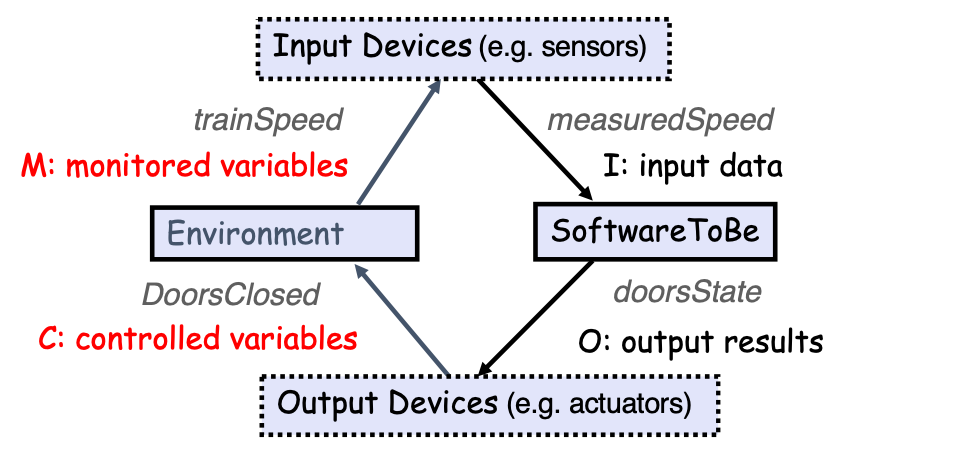
\includegraphics[scale=0.3]{img/modello4.png}
    \label{fig:req_rel}
\end{figure}
Quando parliamo di requisiti software abbiamo questo modello quaternario.
Possiamo avere degli \textit{input device} e degli \textit{output device} che
sono i componenti che permettono di far si che il software possa 
interagire con il mondo reale. 

\subsubsection{Mappatura dei requisiti software e dei requisiti di sistema}
Se i requisiti software sono soddisfatti, le assunzioni sono soddisfatte e 
le proprietà di dominio sono soddisfatte, allora i requisiti di sistema
sono soddisfatti. 
\[
\texttt{SOFREQ}, \texttt{ASM}, \texttt{DOM} \models \texttt{SYSREQ}
\]
\section{Categorie di requisiti}
I requisiti possono essere classificati in base a diverse categorie:
\begin{itemize}
    \item \textbf{Funzionali}: sono frasi che raccontano quelle che sono 
    le funzionalità che il software dovrà fornire per soddisfare i bisogni
    del cliente. Catturando il funzionamento del sistema software.
    \item \textbf{Non funzionali}: sono frasi che raccontano le proprietà
    del sistema software che non sono legate alle funzionalità. Sono quindi
    legati alla qualità del software. Ad esempio, la sicurezza, la 
    performance, la scalabilità, \dots
\end{itemize}
I requisiti non funzionali, essendo un po' trasversali, potrebbero non emergere 
direttamente dagli stakeholder, quindi è opportuno adottare delle tassonomie 
per poterli identificare.
Possono essere raccolti mediante domande esplicite mediante interviste,
questionari, \dots
\section{Il ciclo di vita dei requisiti}
\subsection{Comprensione del dominio}
Prima di tutto è necessario far un passaggio di comprensione del dominio, 
in modo da comunicare con i committenti e gli stakeholder con la terminologia e 
la comprensione del dominio stesso. 
Principalmente si studia il \textit{system as-is} e si cerca di capire come funziona 
il mondo prima che il software venga implementato. Studiando quindi l'organizzazione,
studiando i ruoli, le prassi e individuando i problemi e le opportunità.
Si identificano gli stakeholder e si cerca di capire quali sono i loro bisogni e
le loro aspettative.

\begin{tcolorbox}[colback=yellow!5!white,colframe=yellow!75!black]
Ciò che viene prodotto da questa prima fase è un primo glossario della terminologia
del dominio.
\end{tcolorbox}

\subsection{Elicitazione dei requisiti}
In questa fase si può iniziare ad esplorare il problema che il software 
dovrà risolvere. Capendo le specifiche esigenze degli stakeholder, le opportunità 
tecnologiche e le limitazioni. 
\subsection{Valutazione e negoziazione}
A questo punto possiamo raggiungere il primo target 
dei requisiti concordati con gli stakeholder.
Per raggiungere questo obiettivo, ci sarà, ovviamente una prima fase di negoziazione, 
dove emergeranno i punti di disaccordo tra le varie parti e iniziare a mediare 
tra essi trovando una possibile soluzione.

Tipicamente nella fase di raccolta dei requisiti, si raccolgono anche 
obiettivi contrastanti tra le diverse classi di stakeholder.
Ad esempio alcune responsabilità potrebbero essere volute in capo a parti diverse.

\begin{tcolorbox}[colback=red!5!white,colframe=red!75!black]
    Ciò che viene prodotto da questa fase è un primo documento di
    specifica dei requisiti. 
\end{tcolorbox}

\subsection{Specifica e documentazione}
La fase successiva è quella di documentare tali requisiti con le varie modalità 
per fissarli in maniera formale.
Il documento dei requisiti deve essere un documento strutturato e  deve essere 
redatto in modo che sia comprensibile da tutti gli attori coinvolti.

\begin{tcolorbox}[colback=green!5!white,colframe=green!75!black]
    Ciò che viene prodotto da questa fase è un documento di specifica dei requisiti.
\end{tcolorbox}
\subsection{Consolidamento dei requisiti}
La fase successiva è la fase di validazione e verifica, in modo da poter
capire se è corretto e completo. In modo da capire se abbiamo lacune, inconsistenze
e ambiguità.
Per far ciò ci sono diverse tecniche per:
\begin{itemize}
    \item Validare i requisiti: capire se i requisiti danno risposta concreta e 
    completa a quelle che sono le necessità degli stakeholder.
    \item Verificare i requisiti: capire se sono presenti inconsistenze o lacune 
    nei requisiti.
    \item Dovrà essere verificato rispetto a target qualitativi.
    \item I problemi trovati vanno risolti.
\end{itemize}

\begin{tcolorbox}[colback=blue!5!white,colframe=blue!75!black]
    Ciò che viene prodotto da questa fase è un documento di specifica dei requisiti
    consolidato.
\end{tcolorbox}

Il documento dei requisiti consolidato può fornire una base per la pianificazione 
del piano di test di \textbf{accettazione}. Definendo gli scenari in cui è possibile 
decidere se il software è completo o meno. Sono quindi \textbf{scenari} di alto 
livello.
È possibile, inoltre, abbozzare un piano di test sviluppo.

Tale documento può essere utilizzato come base per la definizione di un contratto 
di fornitura del software.

\subsubsection{La spirale dei requisiti}
Nella prassi si adotta un approccio iterativo e incrementale, in modo da poter
affinare i requisiti in base alle informazioni che si acquisiscono nel tempo.
\begin{figure}[H]
    \centering
    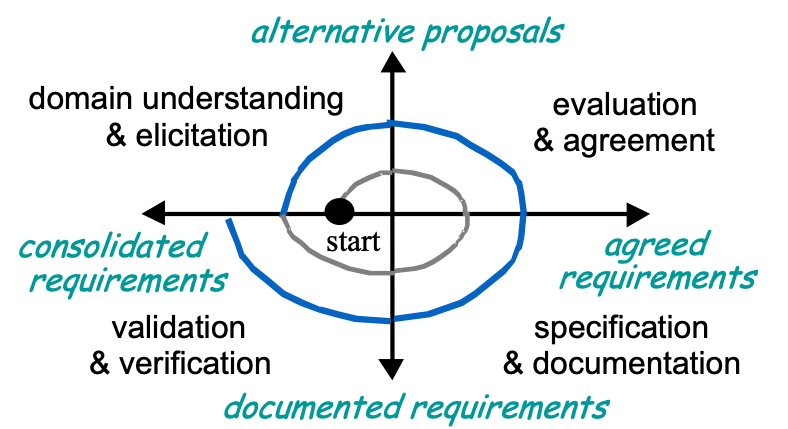
\includegraphics[scale=0.4]{img/ciclo.png}
    \label{fig:ciclo}
\end{figure}
Una visione evolutiva dei requisiti, che si adatta ai mutamenti
dell'ambiente di lavoro,
è caratteristica dello sviluppo agile del software.
\section{Target qualitativi dei requisiti}
I target di qualità, che verranno approfonditi in seguito, sono:
\begin{itemize}
    \item \textbf{Completezza} degli obiettivi, dei requisiti e delle assunzioni
    \item \textbf{Coerenza} degli elementi del documento dei requisiti
    \item \textbf{Adeguatezza} dei requisiti, delle assunzioni e delle proprietà del dominio
    \item \textbf{Chiarezza} degli elementi del documento dei requisiti 
    \item \textbf{Misurabilità} dei requisiti e delle assunzioni
    \item \textbf{Pertinenza} dei requisiti e delle assunzioni
    \item \textbf{Fattibilità} dei requisiti
    \item \textbf{Comprensibilità} degli elementi del documento dei requisiti
    \item \textbf{Buona strutturazione} del documento dei requisiti
    \item \textbf{Modificabilità} degli elementi del documento dei requisiti
    \item \textbf{Tracciabilità} degli elementi del documento dei requisiti
\end{itemize}
\subsection{Errori comuni}
Ci sono varie tipologie di errori che non devono essere commessi:

Tra questi troviamo:

\begin{itemize}
    \item \textbf{Omissione}: l'assenza di requisiti critici rappresenta un errore grave.
    \item \textbf{Contraddizione}: la presenza di requisiti che si contraddicono tra loro costituisce un errore critico.
    \item \textbf{Inadeguatezza}: requisiti che non soddisfano le necessità o gli standard previsti sono considerati errori critici.
    \item \textbf{Ambiguità}: requisiti poco chiari o interpretabili in modi diversi sono errori gravi.
\end{itemize}

Altri problemi comuni includono:

\begin{itemize}
    \item \textbf{Inmisurabilità}: requisiti che non possono essere misurati o quantificati.
    \item \textbf{Rumore e sovraspecificazione}: dettagli superflui o eccessivi che complicano il documento dei requisiti.
    \item \textbf{Infattibilità}: requisiti che non possono essere realizzati, spesso dovuti a pensieri desiderativi.
    \item \textbf{Inintelligibilità}: requisiti che non sono chiari o comprensibili.
    \item \textbf{Scarsa strutturazione}: problemi nella struttura del documento, come riferimenti anticipati o errori di organizzazione.
    \item \textbf{Opacità}: mancanza di trasparenza o chiarezza nei requisiti.
\end{itemize}

\subsection{Il processo di ingegneria dei requisiti può variare a seconda del
tipo di progetto}

Il processo di ingegneria dei requisiti può variare significativamente in base
al tipo di progetto. Alcuni dei principali fattori di variazione includono:

\begin{itemize}
    \item \textbf{Progetti green-field} vs. \textbf{Progetti brown-field}: I
    progetti green-field partono da zero, mentre i progetti brown-field riguardano
    l'aggiornamento o l'espansione di sistemi esistenti.
    \item \textbf{Progetti guidati dal cliente} vs. \textbf{Progetti guidati dal
    mercato}: I progetti guidati dal cliente si concentrano sulle specifiche
    esigenze di un cliente particolare, mentre i progetti guidati dal mercato
    mirano a soddisfare le esigenze generali del mercato.
    \item \textbf{Progetti in-house} vs. \textbf{Progetti esternalizzati}: I
    progetti in-house sono sviluppati internamente all'organizzazione, mentre
    quelli esternalizzati vengono affidati a fornitori esterni.
    \item \textbf{Progetti single-product} vs. \textbf{Progetti product-line}:
    I progetti single-product riguardano un singolo prodotto, mentre i progetti
    product-line coinvolgono una linea di prodotti correlati.
\end{itemize}

I fattori di variazione includono:

\begin{itemize}
    \item Il peso relativo di attività come l'elicitation, la valutazione,
    la documentazione, il consolidamento e l'evoluzione.
    \item L'intreccio tra ingegneria dei requisiti e design.
    \item Il peso relativo dei requisiti funzionali rispetto a quelli non
    funzionali.
    \item I tipi di stakeholder e sviluppatori coinvolti.
    \item Gli usi specifici del documento dei requisiti.
    \item L'uso di tecniche specifiche.
\end{itemize}

\section{Ostacoli nell'ingegneria dei requisiti}
Di fatto l'ingegneria dei requisiti è una disciplina molto complessa,
che si trova ad affrontare diversi ostacoli. Il costo di identificare 
e correggere errori nei requisiti aumenta con il tempo, quindi è
importante riuscire a identificarli il prima possibile.
I costi in fasi avanzate possono arrivare anche a $200$ volte il costo  
di identificazione in fase iniziale.

\subsection{Ostacoli alla buona pratica dell'ingegneria dei requisiti}

Ci sono diversi ostacoli che possono impedire una buona pratica dell'ingegneria
dei requisiti. Tra questi troviamo:

\begin{itemize}
    \item \textbf{Gli sforzi nell'ingegneria dei requisiti sono spesso spesi
    senza la garanzia che il contratto del progetto venga concluso}: Ciò significa
    che una quantità significativa di lavoro può essere svolta senza avere la
    certezza che il progetto andrà effettivamente avanti.
    
    \item \textbf{Pressione su scadenze strette, costi a breve termine e
    aggiornamenti tecnologici}: Le tempistiche ridotte, i vincoli economici
    e la necessità di mantenere il passo con la tecnologia possono mettere
    sotto pressione il processo di ingegneria dei requisiti, portando a compromessi
    nella qualità.
    
    \item \textbf{Scarsa disponibilità di studi sull'economia dell'ingegneria
    dei requisiti}: Esiste una mancanza di dati quantitativi sui benefici e
    sui risparmi dei costi derivanti dall'ingegneria dei requisiti, rendendo
    difficile misurare il progresso rispetto alle fasi di progettazione e
    implementazione.
    
    \begin{itemize}
        \item Mancanza di dati quantitativi sui benefici e sui risparmi dei
        costi dell'ingegneria dei requisiti.
        \item Il progresso nel processo di ingegneria dei requisiti è più
        difficile da misurare rispetto alla progettazione e all'implementazione.
    \end{itemize}
    
    \item \textbf{I documenti dei requisiti sono talvolta percepiti come}: 
    \begin{itemize}
        \item Grandi, complessi e rapidamente obsoleti.
        \item Troppo distanti dal prodotto eseguibile che i clienti stanno pagando.
    \end{itemize}
\end{itemize}
\subsection{Sviluppo Agile e Ingegneria dei Requisiti}

Lo sviluppo agile può superare alcuni degli ostacoli associati all'ingegneria
dei requisiti. Alcuni dei modi in cui lo sviluppo agile riesce a farlo includono:

\begin{itemize}
    \item \textbf{Un maggiore sviluppo agile può superare alcuni ostacoli}:
    \begin{itemize}
        \item Fornendo in modo continuo e precoce funzionalità di valore per
        il cliente.
        \item Riducendo la distanza tra i requisiti e il codice.
    \end{itemize}
    
    \item \textbf{Cicli brevi di ingegneria dei requisiti nel processo a spirale,
    ciascuno seguito direttamente da un breve ciclo di implementazione}:
    \begin{itemize}
        \item Gli incrementi funzionali utili vengono ricavati direttamente
        dall'utente.
        \item Le fasi di valutazione, specifica e consolidamento sono spesso
        abbreviate (ad esempio, la specifica equivale a un caso di test
        sull'implementazione).
        \item Gli incrementi vengono implementati e testati da un piccolo
        team nello stesso luogo, vicino all'utente per un feedback immediato,
        utilizzando regole rigorose.
    \end{itemize}
\end{itemize}
\subsection{Assunzioni forti per il successo dell'agilità}

Perché l'agilità abbia successo, sono necessarie alcune assunzioni forti.
Queste includono:

\begin{itemize}
    \item \textbf{Tutti i ruoli degli stakeholder sono riducibili a un singolo
    ruolo}: Questo implica che le responsabilità e i compiti possono essere
    gestiti da un'unica figura.
    
    \item \textbf{Il progetto è sufficientemente piccolo da essere assegnabile
    a un singolo team di piccole dimensioni, localizzato in un unico luogo}:
    Questo team include programmatori, tester e manutentori.
    
    \item \textbf{L'utente può interagire prontamente ed efficacemente}: La
    comunicazione con l'utente deve essere rapida e produttiva.
    
    \item \textbf{La funzionalità può essere fornita rapidamente, costantemente
    e in modo incrementale, dalle parti essenziali a quelle meno importanti}: Non
    è necessaria la prioritizzazione delle funzionalità.
    
    \item \textbf{Gli aspetti non funzionali, le assunzioni sull'ambiente, gli
    obiettivi, le opzioni alternative e i rischi possono ricevere poca attenzione}:
    Questi elementi sono considerati meno critici.
    
    \item \textbf{Poca documentazione è richiesta per la coordinazione del lavoro
    e la manutenzione del prodotto}: La precisione dei requisiti non è essenziale;
    la verifica prima della codifica è meno importante di un rilascio anticipato.
    
    \item \textbf{Le modifiche ai requisiti non richiedono probabilmente un
    rifacimento significativo del codice}: Le modifiche ai requisiti sono
    gestibili senza necessità di grandi ristrutturazioni del codice.
\end{itemize}

\begin{tcolorbox}[colback=green!5!white,colframe=green!75!black]
    Maggiore/minore agilità è raggiungibile con un minore/maggiore peso
    nelle fasi di elicitazione, valutazione, documentazione e consolidamento dei
    cicli di ingegneria dei requisiti.
\end{tcolorbox}